\part{Theory and Background}\label{part:theory}
\chapter{Quantum networking with neutral Rubidium atoms}\label{ch:intro_to_qn}

% the hierarchy is 
% chapter,section,subsection,etc


\section{Intro to quantum networks}
\subsection{Distributed quantum entanglement as a resource}
Quantum entanglement is a phenomenon in which two or more systems can not be correctly described by treating the systems individually. This is equivalent to saying that the quantum state of the system is not factorable into states for each subsystem. For a system composed of subsystems $A$ and $B$ in an entangled state, e.g. two photons,
\begin{equation}
    \rho_{AB} \neq \rho_A \otimes \rho_B
\end{equation}
where $\rho$ is a Hermitian matrix representing the density operator which gives the state, and the right-hand-side (RHS) represents a product state.
In many cases, the entanglement applies only to one particular degree of freedom, such as the spin state of an atom or the polarization of a photon, whereas the other degrees of freedom remain separable and distinguishable, thus they can be factored out of the overall state. However, entanglement can also involve multiple degrees of freedom, such as both the polarization and frequency of photons, which is referred to as hyperentanglement.

In addition to being an active area of fundamental research, quantum entanglement is also a useful resource in applications such as quantum sensing. Typical quantum sensing schemes rely on measuring the phase between two quantum states, for example using a Ramsey-type interference experiment. For such applications, certain quantum entangled states can show advantage over product states inputs, e.g. owing to a phase which evolves more rapidly than for an unentangled system. Two common states of interest for quantum sensing are GHZ states and N00N states:

\begin{align}
    \ket{\psi_{\text{GHZ}}} &= \frac{1}{\sqrt{2}} \left(\ket{0}^{\otimes n} + \ket{1}^{\otimes n}\right) \\
    \ket{\psi_{\text{N00N}}} &= \frac{1}{\sqrt{2}} \left( \ket{n0} + \ket{0n} \right)
\end{align}
    
Another convenient albeit mysterious attribute of quantum entanglement is that it can be created between widely separated systems, including systems which have never directly interacted. Indeed, entanglement has been generated between photons across 100s and even 1000 km \cite{Neumann2022, Yin2020}. This opens up the door for long-range sensing, such as a network of quantum clocks\cite{Kómár2014}, as well as a network of eaves-drop proof secure communication channels. Moreover, across shorter distances, such distributed entanglement may be an enabling technology for scaling quantum computers, using a network of quantum processor modules\cite{Monroe2014modular}. Some of these applications will be discussed in more detail throughout this thesis.

\section{Quantum networking with neutral atom qubits}

A quantum network can be roughly defined as any system of communication channels in which quantum mechanics plays a role to accomplish some non-classical behavior. For the purpose of this thesis, we will usually take a quantum network to imply a more restricted definition, in which $N\geq2$ spatially separated systems containing matter qubits acting as quantum memory are interconnected by quantum entanglement. The most rudimentary architecture within this definition is two spatially separated two-level systems sharing entanglement, say two atoms with entanglement between their hyperfine states-- the exact architecture of interest to this thesis. It is worth noting that despite its simplicity, such a system can still be used to demonstrate several fundamental features and important building blocks for quantum sensing, quantum key distribution, and distributed quantum computing\cite{main2024, drmota2024, Langenfeld2021}.

To date, distributed or remote entanglement has been generated with many different physical platforms, including but not limited to photons, neutral atoms, ions, nitrogen-vacancy centers in diamond, and superconducting qubits. It is still an open question which system(s) will prevail for useful quantum applications such as distributed quantum processing and sensing. However, as this thesis is concerned with remote entanglement between neutral atoms, we will focus on the advantages and disadvantages of that particular platform at present.

Neutral atoms are renowned in the world of qubits for their inherently identical properties between copies of the same atom, long coherence times, and the ability to interact with electromagnetic fields in a variety of different ranges, from microwave to optical. Moreover, techniques for controlling them are relatively mature thanks to decades of progress in the field and technological advancements, e.g. lasers.  However, no platform is without its downsides. Notably, neutral atoms confined in optical potentials typically remain trapped for only tens of seconds\cite{Schymik2021}, necessitating costly time to reload atoms. This is in contrast with solid state qubits which persist indefinitely and ions which can remain trapped for days in deep traps even with room temperature vacuum systems\cite{Wu2021}.

For quantum networking in particular, neutral atoms possess several key attributes. It is well established that atoms make excellent clocks and quantum sensors for a variety of quantities of interest: electric and magnetic fields, acceleration, and gravitational red-shifts \cite{Kumar2017, d’ArmagnacdeCastanet2024, Bothwell2022}, to name just a few. Moreover, neutral atoms are emerging as a top contender for quantum computing, owing to a relatively  straightforward path to scalability of optical trap arrays \cite{PHuft2022, manetsch2024, Pause2024}, high-fidelity gates using architectures based on either fixed atom arrangement \cite{radnaev2024} or flexible qubit connectivity through atom transport\cite{Evered2023}. Thus, it is natural to pursue linking these extant technologies as the quantum IoT ecosystem develops.

\begin{figure}[!ht]
    \centering
    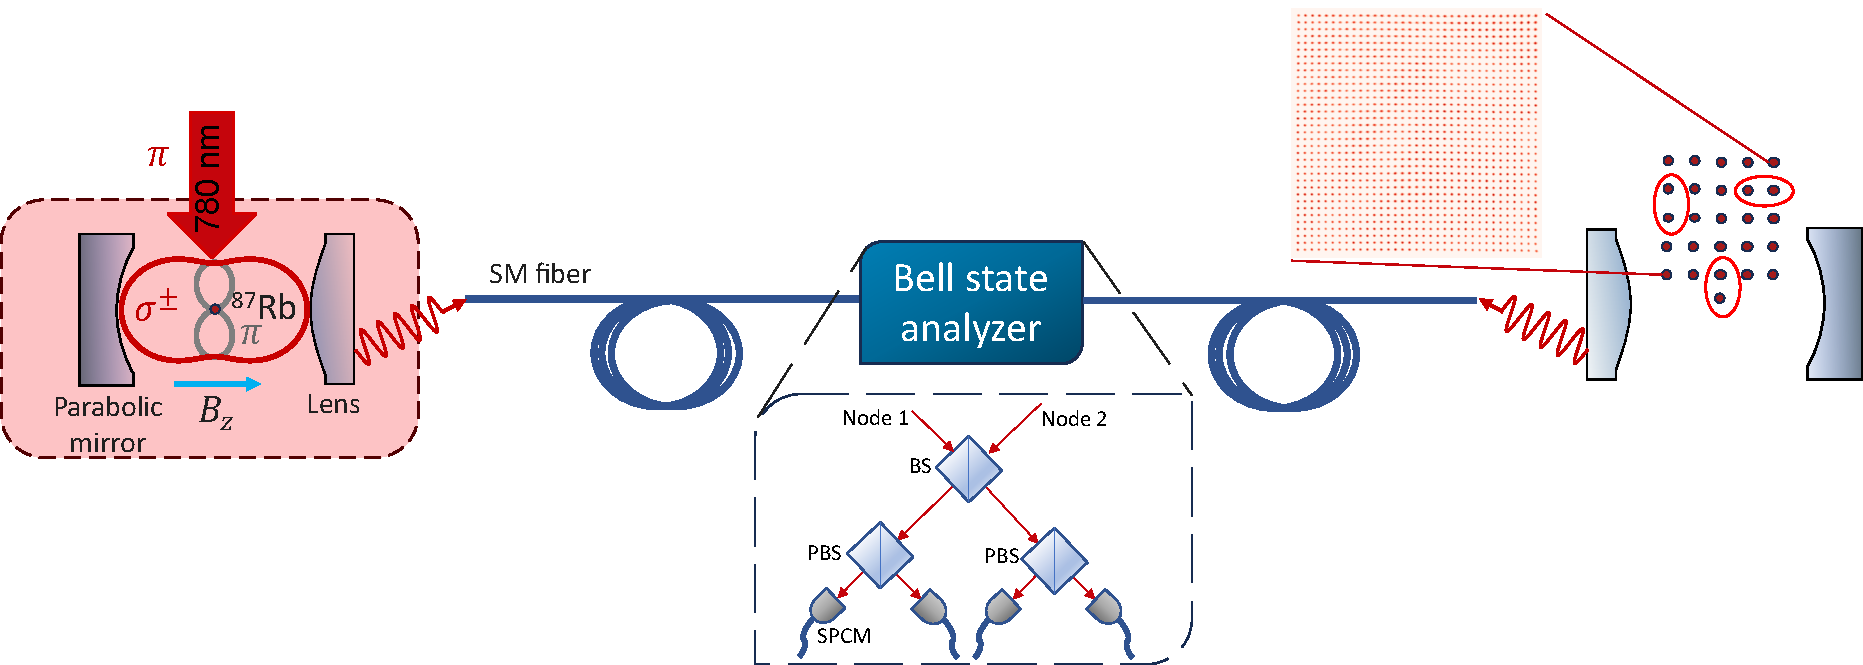
\includegraphics[width=0.9\textwidth]{Images/network_of_quantum_registers.pdf}
    \caption{A rudimentary network of quantum registers as envisioned in this thesis. The red ellipses on the right-hand node represent Rydberg gates between the encircled qubits. The atomic array data inset is from Ch. \ref{ch:array_pra}.}
    \label{fig:quantumnetwork}
\end{figure}

\subsection{Establishing remote entanglement}\label{sec:reg}

Remote entanglement between a pair matter qubits is implemented by intermediate entanglement generation between one or both matter qubits with a flying qubit, or photon. In one class of entanglement schemes, each qubits, say, an atom, is prepared in such a way as to emit a single photon with which it shares entanglement. When a photon from each atom is collected with appropriate optics, the paths of the photons allow them to interfere, entangling the photonic part of the state of the system of atoms and photons. Finally, a measurement is made on the photons which projects entanglement onto the atoms. A simplified version of the relevant optical setup for this entanglement scheme, used in the quantum network described in this thesis, is shown in Fig. \ref{fig:quantumnetwork}. This is an example of entanglement swapping\cite{Zukowski1993}. This scheme is probabilistic as the photons are not collected with unit success probability, but successful entanglement is heralded by the photon detection event.

A second class of remote entanglement schemes involves so-called direct transmission, in which only one atom is entangled with an emitted photon, which is then sent directly to the other atom to be absorbed. This scheme does not always include a heralding event, and can suffer from poor interaction between the photon and receiving atom unless a cavity is used. For the experiment developed for this thesis, the first method of entanglement generation above is the one of interest.

%the chapters and section are not in the best order. this could go before the "establishing remote entanglement section", and all of the sections before "A remote entanglement protocol with Rb" could go in the intro to quantum networks section, with Quantum networking with neutral atom qubits as the final subsection in that section. the new section would be remote entanglement with rb atoms, and the atom-atom rate could be demoted to a subsection   
\subsection{Quantum networks for distributed processing}

Proposals to scale quantum computers with modular approach based on photonic interconnects between processing nodes have been around for over a decade\cite{Monroe2014modular}, and they remain a compelling challenge for the field, with use cases including surface code quantum computing\cite{Horsman2012}. In recent years, there has been an up-tick in both proposals\cite{li2024high, Young2022, Huie2021} and experimental demonstrations\cite{sinclair2024, hartung2024quantum, main2024}, including an industry demonstration with trapped ions\cite{IonQ2024}. For neutral atom based platforms, a good review can be found in \cite{Covey2023}, though it is already slightly outdated. 

As generating remote entanglement is typically probabilistic, and slow compared to other operations on a quantum computer, establishing entanglement between many physical qubits in separate nodes can quickly consume cycle time. Proposals to alleviate this resource strain often involve multiplexing\cite{Huie2021} and iterative approaches to establishing entanglement pairs over multiple attempts\cite{li2024high}. For atomic qubits, the largest gain in entanglement rate is likely to be acheived by enhancing the photon collection efficiency using an optical cavity, which can approach collection efficiencies near unity. As outlined in \cite{Young2022}, using using near-concentric cavities can enable remote entanglement rates on the order of 1000 $\text{s}^{-1}$. Note that the gain for high rate entanglement largely comes in the form of increased link efficiency, as successfully entangled pairs are more likely to remain coherent over the duration of a batch of multi-pair entanglement creation. 

Finally, we note that fidelity in creating remote Bell pairs is typically lower than for controlled gates between qubits in the same node. For example, \cite{saha2024high} showed remote entanglement fidelity of 97$\%$ with ions, whereas local two-qubit gates with ions have exceeded 99.9$\%$ fidelity\cite{harty2014high, ballance2016high, clark2021high,srinivas2021high}. Fortuitously, it turns out that for some approaches to fault-tolerant quantum computing, requirements on fidelity are less stringent for the remote entangled pairs forming the boundary between nodes, tolerating infidelities at the 1$\%$ level\cite{ramette2024fault}.

%now we get specific
\subsection{A remote entanglement protocol with $^{87}$Rb atoms}

The quantum network described in this thesis uses $^{87}$Rb as the matter qubit in each network node involved in entanglement distribution, where a simplified network schematic is shown in Fig. \ref{fig:quantumnetwork}. This choice was made in part to due to its convenient level structure for our choice of entanglement between the spin states of the atom and polarization states of the emitted photon. In what follows, we will describe the remote entanglement protocol in detail.

The remote entanglement generation protocol can be coarsely broken into three chunks. First, a cooled and trapped communication atom at each node is optically pumped into $\ket{5S_{1/2},F=1,m_F=0}$ (Fig. (\ref{fig:entanglement_generation_steps})). Second, the atoms are excited with a $\pi$ pulse to $\ket{5P_{3/2},F=0,m_F=0}$. The atom then undergoes spontaneous emission into three possible decay channels, emitting a photon with either circular polarization $\sigma_{\pm}$ or linear $\pi$. By choosing a quantization axis aligned along the optics which collect the photon and coupling the emission into a single mode fiber, we can restrict the collected photons to only those with circular polarization. This is because the $\pi$-polarized dipole pattern destructively interferes along the quantization axis. Owing to the indistinguishability of the two $\sigma$ decay channels, the collection of a photon results in an atom-photon entangled state given by
\begin{equation}\label{eq:atomphotonstates}
    \ket{\psi^+}=\frac{1}{\sqrt{2}}\left(\ket{m_F=1, \sigma_+}+\ket{m_F=-1,\sigma_-}\right)
\end{equation}
where the phase of the state is fixed by a Clebsch-Gordon coefficient for the decay. Repeated attempts done in parallel to create this state at both nodes until a photon from each node is collected on the same attempt. When this occurs, a joint measurement is done on the photons, which can project the remaining two-atom state into one of two Bell states,
\begin{equation}\label{eq:atomatomstates}
    \ket{\Psi^{\pm}} =\frac{1}{\sqrt{2}}\left(\ket{1,-1}\pm\ket{-1,1}\right)
\end{equation}
with a maximum success probability of $1/2$. The scheme described here was first demonstrated in \cite{Hofmann2012}.

\begin{figure}[!ht]
    \centering
    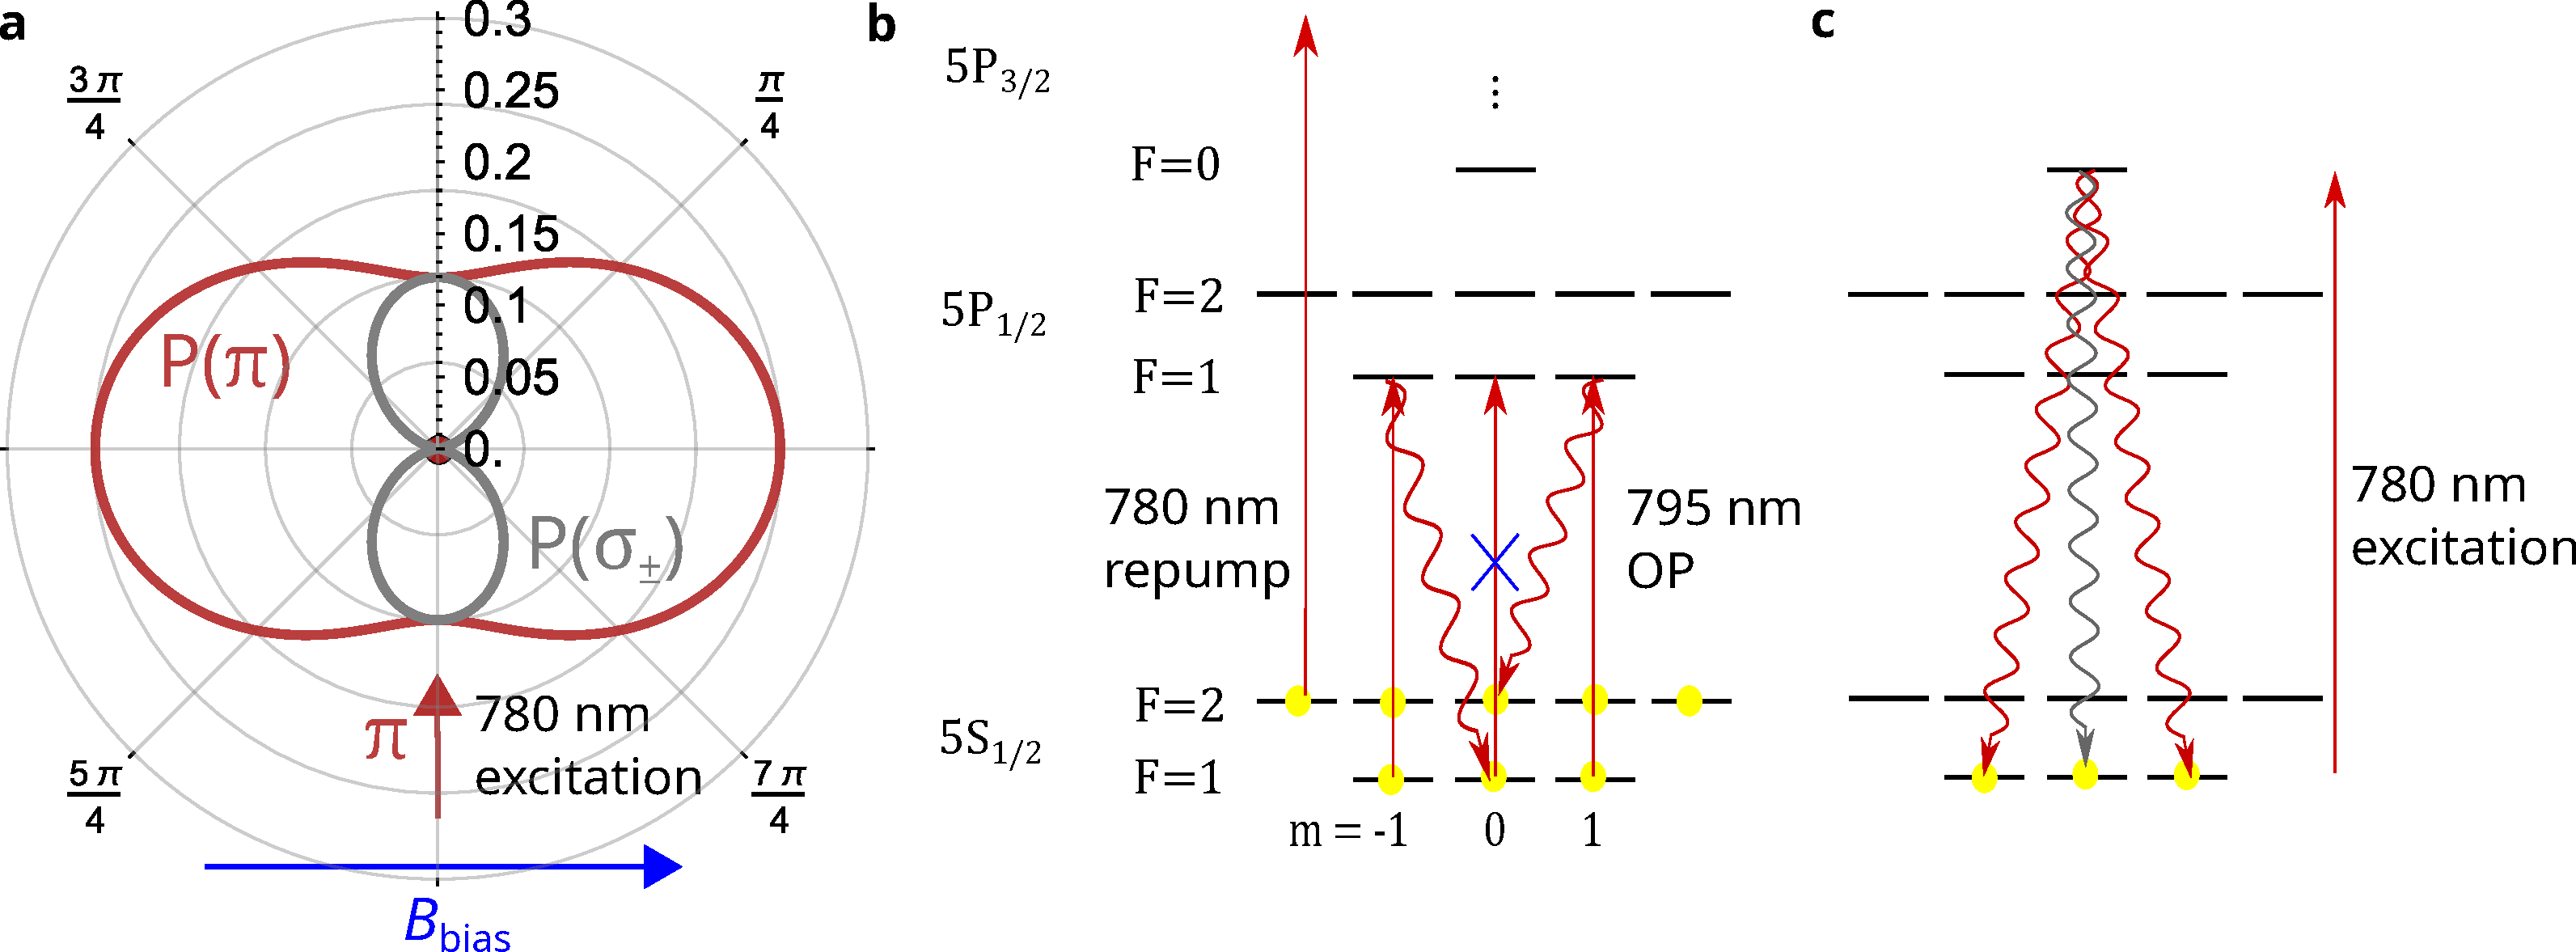
\includegraphics[width=0.9\textwidth]{Images/rb87_atomphoton_entanglement_and_photon_emission_pattern2.pdf}
    \caption{The atom-photon entanglement generation protocol. (a) The dipole emission pattern of the atom, oriented with the quantization axis defined by a magnetic field $B_{\text{bias}}$ aligned to the optical axis of the photon collection optics. (b) The communication atom at each node is optically pumped into $\ket{5S_{1/2},F=1,m_F=0}$, after which (c) the atom is excited with a $\pi$ pulse to $\ket{5P_{1/2},F=0,m_F=0}$, resulting in the creation of an atom-photon entangled state.}
    \label{fig:entanglement_generation_steps}
\end{figure}

% \subsection{Integrating quantum processing arrays with network nodes}
\section{Atom-atom entanglement rate}\label{sec:entanglementrate}

The entanglement protocol described above is probabilistic and requires many attempts per heralded remote entanglement event, predominantly limited by the efficiency of the photon collection optics. It is important to estimate the expected remote entanglement generation (REG) rate, as this will affect what the entanglement resource can be used for. For example, if the REG rate much greater than the decoherence rate of the entangled state, we can generate many entangled pairs in succession, which may be a requirement for some entanglement purification protocols as well as quantum sensing.

The per-attempt success probability of REG, i.e. atom-atom entanglement, is given simply by
\begin{equation}
    P_{\text{aa}} = \frac{1}{2}P_{\text{ap}}^2
\end{equation}
where $P_{\text{ap}}$ denotes the one-node atom-photon entanglement success probability and the factor of $1/2$ results from only two out of four Bell states being able to be distinguished by the photonic Bell state measurement. $P_{\text{ap}}$ is limited by the photon collection efficiency of per excitation attempt $\eta_{\text{col}}$ and the detection efficiency $\eta_{\text{det}}$. All losses from optical alignment, finite transmission through optical elements including absorption in optical fiber, and detector efficiency can be lumped into these two quantities, so we can write 
\begin{equation}
    P_{\text{aa}} = \frac{1}{2}\left(\eta_{\text{col}}\eta_{\text{det}}\right)^2
\end{equation}
where it has been assumed that the collection and detection efficiency are the same for each node. Additional losses such as imperfect success probability in initializing the atom state and exciting it have been ignored, but these could be accounted for by including them in $\eta_{\text{col}}$.

The rate of REG depends on the atom-photon entanglement attempt rate and the duty cycle of the attempt loop (Fig. (\ref{fig:REG_loop})), such that the average REG rate is given by
\begin{equation}\label{eq:Raa}
    R_{\text{aa}} = \eta_{\text{duty}}R_{\text{attempt}}P_{a   a} = \bar{R}_{\text{attempt}}P_{\text{aa}}
\end{equation}
where $\bar{R}_{\text{attempt}}$ is the average attempt rate. The duty cycle $\eta_{\text{duty}}$ is to some extent platform dependent. For example, neutral atoms can occasionally be lost from the trap either through heating during the excitation loop or by collisions with background atoms, necessitating a break in the loop for reloading an atom which can take 100s of ms. For platforms such as ions and NV centers this kind of break is not needed. It is worth noting however that the REG rate reported in literature does not always take into account the duty cycle of the excitation loop, such as in \cite{Young2022}, such that the reported rate is really max rate rather than the average rate. Whether this distinction is important is likely application dependent, but it is clear that a high rate REG loop broken up by large amounts of downtime could be severely limiting.

\begin{figure}[!ht]
    \centering
    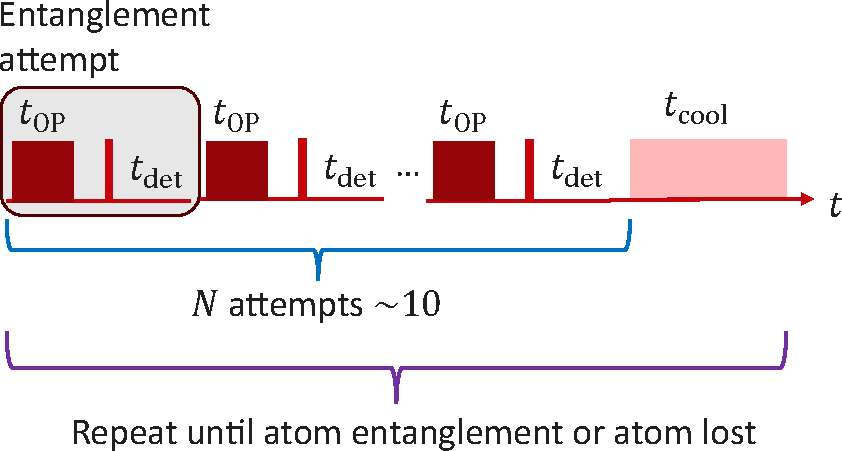
\includegraphics[width=0.5\textwidth]{Images/entanglement_attempt_loop.pdf}
    \caption{The remote entanglement generation loop.}
    \label{fig:REG_loop}
\end{figure}

The attempt rate $R_{\text{aa}}$ can be estimated given the duration of the different elements of the experiment sequence together with assumptions for the atom lifetime in the trap and heating rate. The entanglement attempt loop sequence is shown in Fig. \ref{fig:REG_loop}, and consists of optical pumping and excitation phases interspersed with Doppler re-cooling to alleviate atom heating, as well as atom reloading triggered by the absence of an atom signal during re-cooling. To write down the attempt rate, we first define the following quantities:
\begin{align}
    N_{\text{total}} &= \frac{1}{P_{\text{aa}}} \\
    N_{\text{epoch}} &= \frac{N_{\text{total}}}{N_{\text{series}}}.
\end{align}
The first line gives the mean number of tries per REG success, and second gives the number entanglement "epochs", where one epoch is defined as a sequence of entanglement attempts followed by one Doppler re-cooling phase. $N_{\text{series}}$ is the number of entanglement attempts (optical pumping follwed by excitation pulse) we can do in series with re-cooling, i.e. the number of attempts per epoch. Using these definitions, the mean time per remote entanglement success during the attempt loop is 
\begin{equation}
    t_{\text{aa}}=\frac{t_{\text{aa}}^{(\text{loop})}}{\eta_{\text{duty}}}=\frac{1}{\eta_{\text{duty}}}N_{\text{epoch}}\left(N_{\text{series}}\left(t_{\text{OP}} + t_{\pi} + t_{\text{det}}\right) + t_{\text{cool}}\right)
\end{equation}
where the subscripted times denote the optical pumping, $\pi$-pulse excitation, detection, and Doppler re-cooling durations. This gives the REG rate that appears in Eq. (\ref{eq:Raa}) as $R_{\text{aa}} = \eta_{\text{duty}}/t_{\text{aa}}^{(\text{loop})}$. For realistic parameters (see Table \ref{tab:entanglement_steps}), we can compute $P_{\text{aa}}$ and $R_{\text{aa}}$.
\begin{sidewaystable}
% \begin{table}[h!] % too wide
    \centering    
    \begin{tabular}{llll}
        \hline Operation & Label & Duration & Success probability \\
        \hline (a) Entanglement generation: & & & \\
        1- prepare MOT, load into dipole trap & $t_{\textrm{load}}$ & 500 ms & $>0.99$ \\
        2- pump to $5 s_{1 / 2}\ket{1,0}$ & $t_{\textrm{OP}}$ & $6 ~\mu \mathrm{s}$ & $>0.99$ \\
        3- $\pi$-pulse to $5 p_{3 / 2}\ket{0,0}$ & $t_\pi$ & 30 ns & $>0.99$ \\
        4a- atomic decay, record and process photon clicks & $t_{\text {det }}$ & $1 ~\mu \mathrm{s}$ & 1 \\
        4b- cool atom if proper coincidence is not registered after $N_1=10$ cycles & $t_{\textrm{cool}}$ & $100 ~\mu \mathrm{s}$ & $>0.99$ \\
        (b) Entanglement verification: & & & \\
        5- map atomic qubit states $\ket{1,1} \rightarrow \ket{2,1}$ with $\mu$-wave $\pi$-pulse & $t_{\mu \textrm{w}}$ & $50 ~\mu \mathrm{s}$ & $\sim 0.99$ \\
        6- atomic qubit rotation with $\mu$-wave $+\mathrm{RF}~\pi / 2$ pulse & $t_{\mathrm{rot}}$ & $500 ~\mu \mathrm{s}$ & $\sim 0.98$ \\
        7- non-destructive atomic state measurement & $t_{\textrm{m}}$ & 3 ms & $\sim 0.94$\cite{Kwon2017} \\
        8- cool atom to maintain localization in trap & $t_{\textrm{cool}}$ & $100 ~\mu \mathrm{s}$ &$>0.99$ \\
        \hline
    \end{tabular}
    \caption{Entanglement generation and tomography operations and estimates of their durations, adapted from \cite{Young2022}.}
    \label{tab:entanglement_steps}
% \end{table}
\end{sidewaystable}
\newpage

Although we can reuse atoms by re-cooling between successive entanglement attempts, eventually an atom will be lost due to a collision with background atoms. We can expect an average number of entanglement events before needing to reload an atom given by 
\begin{equation}
    N_{\text{aa}} = \frac{\tau_{\text{trap}}}{t_{\text{aa}}}
\end{equation}
where $\tau_{\text{trap}}$ is the lifetime of the atom in the dipole trap. This can be though of as an upper bound, as experiments in which the entanglement is used for something, e.g. for sensing, will likely need to reload atoms more often. State-of-the-art experiments have shown trap lifetimes of 1000s of seconds in cryogenic environments \cite{Schymik2021}, and typically $\sim10$ s at room temperature using two-chamber systems \cite{Graham2022}. However, for the experiment described in this thesis where the MOT is loaded from a background vapor, $\tau_{\text{trap}}$ is around 2 s.

\subsection{Link efficiency}
Another important quantity of interest for generating distributed entanglement is the link efficiency, given by the ratio of the REG rate to the entangled state decoherence rate, or equivalently the coherence time over the mean time per REG:
\begin{equation}
    \eta_{\text{link}} = \frac{R_{\text{aa}}}{\gamma_{\text{coh}}} = \frac{T_2^*}{t_{\text{aa}}}.
\end{equation}
If we imagine a two-node network which can only create entanglement pairs in series, $\eta_{\text{link}}=1$ would imply that an entangled state has decohered by the time a subsequent state can be created. To date, $\eta_{\text{link}}>1$ has been out of reach for many experimental demonstrations, as shown in Fig. \ref{fig:covey_link_eff}.

% could add more recent results to the plot?
\begin{figure}[!ht]
    \centering
    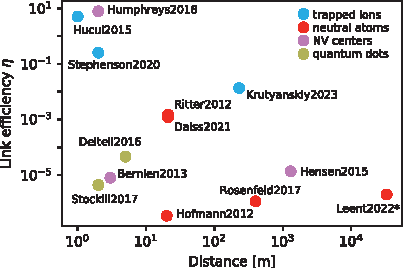
\includegraphics[width=0.7\textwidth]{Images/covey_link_efficiency.pdf}
    \caption{Link efficiency for rudimentary quantum  networks vs the node separation across different platforms, reproduced from \cite{Covey2023}}
    \label{fig:covey_link_eff}
\end{figure}

% \subsection{Photon collection - optical cavity vs free-space}
% % could mention assumption of negligible dark rates, then lift this assumption later.
% \subsection{Experiment repetition rate}
\section{Entanglement fidelity}

\subsection{Dominant contributions}
% dark counts effect fidelity and quantum efficiency effect the rate, 
% but I discuss both effects here

There are multiple sources which contribute to the infidelity of a remote entangled state, some of which arise from infidelity sources for the atom-photon entanglement state at each node, and some of which are related specifically to the atom-atom state. There are several sources which go over the main points in detail, and I will not attempt to repeat this here. An overview of infidelity estimates specific to the entanglement scheme with $^{87}$Rb presented here, including effects which arise if photons are collected with a cavity rather than free-space optics, is given in\cite{Young2022}. I will go over some of these, but only in brief, as they are beyond the concern of the scope of the experimental results presented in this thesis.

Sources of infidelity specific to the creation of the atom-photon entangled state include collecting photons of unwanted polarization, dephasing of the atomic qubit, and off-resonant excitation. The latter two are essentially negligible, but the polarization has to be carefully controlled. As there are three decay channels from $F=0, m=0$ (Fig. (\ref{fig:entanglement_generation_steps}c)), and we only want a state which includes the $\sigma$-polarized components of the emission, it is important not to collect the $\pi$ component. This is accomplished if the optical collection axis coincides with the quantization axis set by a magnetic bias field, and the collected photons are coupled into a single mode fiber.

Both the atom-photon and atom-atom entanglement fidelity are affected by dark counts from the dark detector, which should be negligible. For those used in the experiment described (Laser Components COUNT NIR), the rate is 50 s$^{-1}$, which corresponds to a mean of $5\cdot 10^{-7}$ dark counts in a 100 ns collection window, compared to odds of order $\sim$0.05 of detecting a photon from the atom -- a signal to noise of $10^5$.

Multi-photon scattering is not a problem for our entanglement protocol, if the bias field is set correctly as discussed above, as only $\pi$-polarized emission back into $\ket{F=1,m=0}$, which is not collected, can lead to a second excitation event during the excitation pulse. Put another way, detection of a photon implies $\sigma$-polarization, such that amplitude for re-excitation is projected to zero. The re-excitation process can, however, lead to jitter in the arrival time of photons which affects the contrast of interference of photons from each node, but this is expected to be a small effect.

Mismatch in temporal, or equivalently frequency, overlap of photons from both nodes at the Bell state analyzer will degrade the atom-atom entanglement fidelity, scaling with the overlap of the wavepackets in time. This mismatch can be caused by differences in the arrival time of photons, as well as differences in their carrier frequencies or bandwidths. The former can be adjusted through the experimental control sequence timing in software and by adjusting cable and optical path lengths. The bandwidth of the photons is determined by the atomic linewidth. Any difference in carrier frequency of photons is determined by the bias field at the atoms which sets the quantization axis, and it is imperative that this difference is small compared to the transition linewidth. Imagining the overlap of the photons in frequency space is helpful for having an intuitive foothold. For a bias field of order $\sim1$ G, there will be a relative shift $\Delta$ of order $\sim2\pi\times1$ MHz between $\sigma_+$ and $\sigma_-$ photons due to the hyperfine Zeeman shifts, which is comparable to the $6$ MHz linewidth of the $5P_{3/2}$ states. This will lead to reduced Hong-Ou-Mandel contrast, but contrast can be recovered by limiting the detection window to be $< 2\pi/\Delta$, which is satisfied with a detection window of $\sim100$ ns. This arises from the time-frequency uncertainty relation for the measurement.

\subsection{Smaller effects}
\subsubsection{Polarization change from parabolic mirror}

Polarized light reflected from a surface will in general accrue a phase shift and reduction in amplitude, both of which depend on the angle of incidence and whether the polarization is perpendicular to the surface (S-polarized) or parallel to the surface (P-polarized). Both of these effects will lower the fidelity of our atom-photon entangled state, which uses a circular polarization encoding, but we will show that this is not expected to be a significant source of infidelity.

From \cite{fowles1989introduction}, the reflection amplitudes for S- and P-polarized light at a vacuum-metal boundary are given by
\begin{align}
    r_s &= \frac{\cos(\theta)-n\cos(\phi)}{\cos(\theta)+n\cos(\phi)} \\
    r_p &= \frac{-n\cos(\theta)+\cos(\phi)}{n\cos(\theta)+\cos(\phi)}
\end{align}
where $\phi = \sin^{-1}(\theta/n)$, $\theta$ is the angle of incidence, and $n$ is the complex index of refraction. The parabolic mirror used in the experiments discussed here is coated with silver, for which $n=0.033687+i 5.4208$ for 780 nm light.

Circularly polarized light, e.g. right-handed, can be written as
\begin{equation}
    \textbf{E}_{\textrm R} = E_0 \hat{e}_{\textrm p} + i E_0 \hat{e}_{\textrm s}
\end{equation}
where the $\hat{e}_{\textrm i}$ are unit vectors. After reflection, this becomes
\begin{equation}
    \textbf{E}_{\textrm R} = E_0 r_{\textrm p} \hat{e}_{\textrm p} + i E_0 r_{\textrm s} \hat{e}_{\textrm s}.
\end{equation}
We can now compute the fidelity of the reflected state to the input state in terms of the angle of reflection. Light emitted from an atom trapped at the focus of the parabolic mirror will be incident on the mirror at some angle $\theta_i$ w.r.t. the surface normal for a given emission angle $\theta$ from the optical axis. Because the reflected rays are parallel to the optical axis for an emitter at the mirror focus, $\theta_i=\theta/2$. The maximum angle is related to the clear aperture (CA) radius $\rho_{\textrm CA}$ by 
\begin{equation}
    \theta_{\textrm CA} = \tan^{-1}
    \left(\frac{\rho_{\textrm CA}}{f-\rho_{\textrm CA}^2/(4f)}\right)
\end{equation}
where $f=5.26$ mm is the mirror focal length. Finally, including a weighting function $f(\theta)$ for the emission intensity pattern, we have the fidelity of the reflected polarization state to the input state given by
\begin{equation}
    \mathcal{F} = \frac{\int_0^{ \theta_{\textrm CA}} \left|\frac{1}{2}(\hat{e}_{\textrm p} + i \hat{e}_{\textrm s})\cdot(r_{\textrm p}(\theta') \hat{e}_{\textrm p} - i r_{\textrm s}(\theta') \hat{e}_{\textrm s})\right|^2 f(\theta') d \theta'}{\int_0^{ \theta_{\textrm CA}} f(\theta')  d\theta'}.
\end{equation}
For unpolarized emission, the intensity pattern has no $\theta$ dependence so $f(\theta)=1$, resulting in $\mathcal{F}=0.99544$. We expect a marginal increase for emission which is less likely at large $\theta$, where the angle of incidence, and consequently the fidelity reduction, is more appreciable. For $\sigma$ emission with the quantization axis along the mirror, $f(\theta)=1+\cos^2(\theta)$ up to a numerical prefactor, and $\mathcal{F}=0.99545$, which is a negligibly higher than for uniform emission. We can conclude that the action of reflection from the high NA mirror does not contribute substantially to infidelity of the atom-photon Bell state.

% \subsubsection{Raman scattering in optical fibers}

% Does this matter at all?

